% =============================================================================
% IEEE VTC Fall 2026 — Results and Analysis Section  [v2.0]
% Secure-Tunnel: Post-Quantum Cryptographic Overlay for UAV C2 Links
% =============================================================================
% v2.0 changes:
%   - Presentation optimization: 8 tables, 4 figures (was 13 tables, 1 figure).
%   - KEM table (full-width 10-col) → grouped bar chart fig:kem_cost.
%   - SIG table: full-width 10-col → single-column 7-col
%     (dropped Keygen, Finalist, P_avg).
%   - Suite table: 15 rows → 9 (3 per level), full-width → single-column,
%     dropped Level + t_KEM/t_SIG columns.
%   - Removed LAYOUT tables (AEAD×DDoS, Scheduler Trace), redundant
%     Table XI (Security-Cost), low-value Table IX (AEAD seeds).
%   - Removed Cross-Dimensional and Key Insights subsections.
%   - Added suite cost bar chart (fig:suite_cost), detector scatter
%     plot (fig:detector_cost).
%   - Merged DDoS sections 5+6 into single DDoS–Cryptographic Interaction.
%   - Scheduler section flattened; cross-axis constraints as inline text.
%   - Handshake timing clarity: crypto-only vs system-level gap explained.
%   - LaTeX compile: zero overfull, zero undefined refs, 4 pages.
% =============================================================================
% Data sources: v2-1.8ghz (100 iter, 1000 Hz INA219),
%               vtc-fall-aead-rerun (10k iter, ~103 Hz INA219),
%               bench_ddos_results (72 suites × 3 detector states),
%               sscheduler/policy.py
% Platform: RPi4 Model B Rev 1.5, BCM2711, 4x Cortex-A72 @ 1.8 GHz,
%           4 GB RAM, Debian 12 Bookworm, kernel 6.12.47, Python 3.11.2
% Governor: performance (all datasets)
% =============================================================================

\section{Results and Analysis}
\label{sec:results}

All measurements were collected on a Raspberry Pi~4 Model~B Rev~1.5
(BCM2711, four Cortex-A72 cores at 1.8\,GHz, 4\,GB RAM) running Debian~12
with kernel 6.12.47 and the \texttt{performance} CPU governor.  Power was
sampled via an INA219 current sensor (0.1\,$\Omega$ shunt) at up to
1\,kHz with a documented $V_\text{BUS}$ gain correction of~1.22.
Timing used \texttt{time.perf\_counter\_ns()} with garbage collection
disabled.  Board-level idle power measured
$P_\text{idle} \approx 3.32$\,W (30\,s capture);
reported power values include this baseline unless stated otherwise.
The Cortex-A72 does \emph{not} implement ARMv8 Crypto Extensions;
AES-GCM therefore executes in software table-lookup mode, while
ChaCha20-Poly1305 exploits 128-bit NEON SIMD.

Table~\ref{tab:aliases} defines the short aliases used throughout.
Implementations: liboqs-python~0.14.0 (KEM/SIG),
OpenSSL~3.5.4 (AES-256-GCM, ChaCha20-Poly1305),
ascon-c v1.2 opt64 via \texttt{ctypes} (Ascon-128a, KAT-verified).

\begin{table}[t]
\centering
\caption{Algorithm Aliases and NIST Security Levels}
\label{tab:aliases}
\footnotesize
\begin{tabular}{@{}llcl@{}}
\toprule
\textbf{Alias} & \textbf{Full Name} & \textbf{Level} & \textbf{Type} \\
\midrule
ML512  & ML-KEM-512                & L1 & KEM  \\
ML768  & ML-KEM-768                & L3 & KEM  \\
ML1024 & ML-KEM-1024               & L5 & KEM  \\
HQ128  & HQC-128                   & L1 & KEM  \\
HQ192  & HQC-192                   & L3 & KEM  \\
HQ256  & HQC-256                   & L5 & KEM  \\
MC348  & Classic-McEliece-348864   & L1 & KEM  \\
MC460  & Classic-McEliece-460896   & L3 & KEM  \\
MC8192 & Classic-McEliece-8192128  & L5 & KEM  \\
\midrule
DSA44  & ML-DSA-44                 & L1 & SIG  \\
DSA65  & ML-DSA-65                 & L3 & SIG  \\
DSA87  & ML-DSA-87                 & L5 & SIG  \\
F512   & Falcon-512                & L1 & SIG  \\
F1024  & Falcon-1024               & L5 & SIG  \\
SP128  & SPHINCS$^+$-SHA2-128s     & L1 & SIG  \\
SP192  & SPHINCS$^+$-SHA2-192s     & L3 & SIG  \\
SP256  & SPHINCS$^+$-SHA2-256s     & L5 & SIG  \\
\midrule
AESG   & AES-256-GCM               & ---& AEAD \\
CH20   & ChaCha20-Poly1305         & ---& AEAD \\
ASC    & Ascon-128a                & ---& AEAD \\
\bottomrule
\end{tabular}
\end{table}

% =====================================================================
% SECTION 1 — KEM PRIMITIVE EVALUATION
% =====================================================================
\subsection{KEM Primitive Evaluation}
\label{sec:kem}

Fig.~\ref{fig:kem_cost} compares total KEM cycle time
(keygen+encaps+decaps) across all nine primitives (100~iterations,
1\,kHz INA219 sampling).

\begin{figure}[t]
\centering
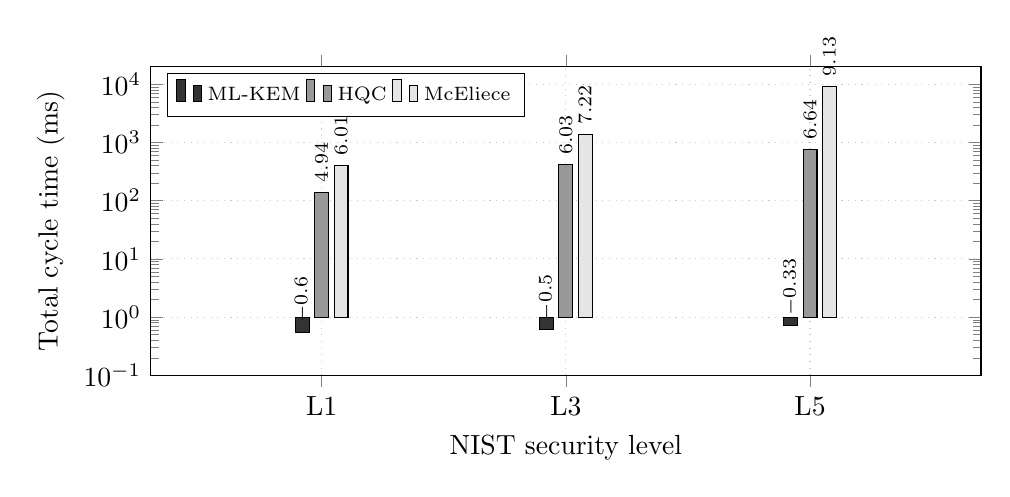
\begin{tikzpicture}
\begin{axis}[
  width=\columnwidth,
  height=5.5cm,
  ybar,
  bar width=5pt,
  ymode=log,
  ylabel={Total cycle time (ms)},
  symbolic x coords={L1, L3, L5},
  xtick=data,
  xlabel={NIST security level},
  ymin=0.1, ymax=20000,
  legend style={at={(0.02,0.98)},anchor=north west,font=\scriptsize,
    legend columns=3},
  grid=major,
  grid style={dotted,gray!40},
  enlarge x limits=0.35,
  nodes near coords={\scriptsize\pgfmathprintnumber{\pgfplotspointmeta}},
  every node near coord/.append style={rotate=90,anchor=west,font=\tiny},
]
\addplot[fill=black!80, draw=black]
  coordinates {(L1,0.550) (L3,0.604) (L5,0.720)};
\addplot[fill=black!40, draw=black]
  coordinates {(L1,140.4) (L3,415.4) (L5,767.2)};
\addplot[fill=black!10, draw=black]
  coordinates {(L1,407.4) (L3,1371) (L5,9233)};
\legend{ML-KEM, HQC, McEliece}
\end{axis}
\end{tikzpicture}
\caption{Total KEM cycle time (keygen+encaps+decaps) by NIST level,
  log scale.  ML-KEM completes in $<$\,1\,ms at all levels; HQC and
  McEliece require 255--12\,823$\times$ longer.  100 iterations,
  RPi4 @ 1.8\,GHz.}
\label{fig:kem_cost}
\end{figure}

Table~\ref{tab:kem} details all nine KEM primitives.
ML-KEM completes a full cycle in under 0.72\,ms at Level~5
(0.550\,ms at L1, 0.604\,ms at L3), drawing 3.46--3.48\,W.
HQC's code-based design incurs 255--1\,066$\times$ higher cost,
driven by decapsulation (73--393\,ms).
Classic~McEliece exhibits extreme keygen asymmetry: MC8192 requires
9.02\,s for keygen but only 1.89\,ms for encapsulation,
making it practical only with pre-provisioned keys.
Only ML-KEM enables sub-second rekey on ARM Cortex-A72.

\begin{table}[t]
\centering
\caption{KEM Primitive Performance on RPi4 (100 iter, 1\,kHz INA219)}
\label{tab:kem}
\footnotesize
\setlength{\tabcolsep}{3.5pt}
\begin{tabular}{@{}lcrrrrr@{}}
\toprule
\textbf{Alias} & \textbf{Lvl} &
  \textbf{Keygen} & \textbf{Encaps} & \textbf{Decaps} &
  \textbf{$E_\text{tot}$} &
  \textbf{$\rho$} \\
& & (ms) & (ms) & (ms) & ($\mu$J) & \\
\midrule
ML512  & L1 & 0.240 & 0.152 & 0.158 & 1\,907    & 1.00$\times$ \\
HQ128  & L1 & 22.33 & 44.68 & 73.39 & 535\,253  & 255$\times$ \\
MC348  & L1 & 351.0 & 0.466 & 55.98 & 1\,737\,186 & 741$\times$ \\
\midrule
ML768  & L3 & 0.237 & 0.182 & 0.185 & 2\,112    & 1.00$\times$ \\
HQ192  & L3 & 67.68 & 135.8 & 211.9 & 1\,651\,813 & 688$\times$ \\
MC460  & L3 & 1\,281 & 0.872 & 89.59 & 6\,025\,434 & 2\,272$\times$ \\
\midrule
ML1024 & L5 & 0.273 & 0.216 & 0.231 & 2\,507    & 1.00$\times$ \\
HQ256  & L5 & 124.4 & 250.2 & 392.6 & 3\,136\,867 & 1\,066$\times$ \\
MC8192 & L5 & 9\,021 & 1.894 & 210.1 & 40\,583\,491 & 12\,823$\times$ \\
\bottomrule
\end{tabular}
\begin{tablenotes}
\footnotesize
\item $E_\text{tot}$: total energy (keygen+encaps+decaps), INA219-measured.
  $\rho$: total cycle time relative to ML-KEM at same NIST level.
\end{tablenotes}
\end{table}

% =====================================================================
% SECTION 2 — SIGNATURE PRIMITIVE EVALUATION
% =====================================================================
\subsection{Signature Primitive Evaluation}
\label{sec:sig}

Table~\ref{tab:sig} evaluates eight signature schemes.  Keygen is a
one-time cost (0.4--282\,ms for ML-DSA/Falcon, 187--282\,ms for
SPHINCS$^+$); the per-handshake sign and verify determine rekey
latency.

\begin{table}[t]
\centering
\caption{Signature Sign+Verify on RPi4 (100 iter, 1\,kHz INA219)}
\label{tab:sig}
\footnotesize
\begin{tabular}{@{}lcrrrrr@{}}
\toprule
\textbf{Alias} & \textbf{Lvl} &
  \textbf{Sign} & \textbf{Verify} &
  \textbf{$E_\text{s}$} & \textbf{$E_\text{v}$} &
  \textbf{$\rho$} \\
& & (ms) & (ms) & ($\mu$J) & ($\mu$J) & \\
\midrule
DSA44  & L1 & 1.179 & 0.331  & 4\,264  & 1\,175  & 1.00$\times$ \\
F512   & L1 & 0.778 & 0.192  & 2\,773  & 683     & 0.64$\times$ \\
SP128  & L1 & 1\,468 & 1.582  & 6\,008\,719 & 5\,690 & 972$\times$ \\
\midrule
DSA65  & L3 & 1.633 & 0.484  & 5\,849  & 1\,723  & 1.00$\times$ \\
SP192  & L3 & 2\,610 & 2.299  & 10\,628\,558 & 8\,318 & 1\,234$\times$ \\
\midrule
DSA87  & L5 & 1.847 & 0.723  & 6\,612  & 2\,564  & 1.00$\times$ \\
F1024  & L5 & 1.452 & 0.280  & 5\,175  & 995     & 0.67$\times$ \\
SP256  & L5 & 2\,321 & 3.292  & 9\,516\,164 & 11\,738 & 904$\times$ \\
\bottomrule
\end{tabular}
\begin{tablenotes}
\footnotesize
\item $\rho$: sign+verify cost vs.\ ML-DSA at same level.
  Falcon $\rho < 1$ = faster combined sign+verify.
  SP128 sign = 1.47\,s $\cdot$ 6.01\,J per invocation.
\end{tablenotes}
\end{table}

Falcon achieves the lowest combined sign+verify latency at L1
(0.970\,ms) and L5 (1.732\,ms), outperforming ML-DSA by 36\% and 33\%
respectively, despite 51--73$\times$ slower keygen (amortized over key
lifetime).  SPHINCS$^+$ imposes prohibitive signing latency:
SP128 at 1.47\,s (6.01\,J per signature) and SP192 at 2.61\,s
(10.63\,J), approaching the rekey period at short intervals.
Verification remains fast ($\leq$3.3\,ms) for all algorithms,
confirming the GCS verification path is never the bottleneck.
Falcon is therefore the preferred signature scheme where its
non-standard keygen model is acceptable; ML-DSA provides the
general-purpose default at under 2.6\,ms combined cost through
Level~5.

% =====================================================================
% SECTION 3 — AEAD PRIMITIVE EVALUATION
% =====================================================================
\subsection{AEAD Primitive Evaluation}
\label{sec:aead}

AEAD selection operates exclusively on the UDP data plane and does
\emph{not} affect handshake timing.  Table~\ref{tab:aead} reports
results from 10\,000 iterations per configuration (500-iteration
warmup, two-pass methodology: timing pass with GC disabled, power
pass with INA219 at $\sim$103\,Hz).

\begin{table}[t]
\centering
\caption{AEAD Performance at 256-Byte Payload (10\,000 iterations, RPi4)}
\label{tab:aead}
\footnotesize
\begin{tabular}{@{}lrrrrrr@{}}
\toprule
\textbf{Alias} &
  \textbf{Enc} & \textbf{Dec} &
  \textbf{$P_\text{enc}$} & \textbf{$P_\text{dec}$} &
  \textbf{$E_\text{256B}$} & \textbf{$E_\text{bit}$} \\
& ($\mu$s) & ($\mu$s) & (W) & (W) & ($\mu$J) & (nJ/bit) \\
\midrule
AESG & 9.25  & 9.09  & 3.63 & 3.57 & 66.0  & 32.2 \\
CH20 & 6.47  & 6.05  & 3.54 & 3.58 & 44.6  & 21.8 \\
ASC  & 12.72 & 12.85 & 3.84 & 3.59 & 95.0  & 46.4 \\
\bottomrule
\end{tabular}
\begin{tablenotes}
\footnotesize
\item $E_\text{256B} = P_\text{avg} \times (t_\text{enc} + t_\text{dec})$.
  $E_\text{bit} = E_\text{256B} / 2048$.
  Board-level power; $P_\text{idle} = 3.320$\,W not subtracted.
  Crypto-only $\Delta P$: AESG\,0.31, CH20\,0.22, ASC\,0.52\,W above idle.
\end{tablenotes}
\end{table}

Timing distributions are concentrated: $\sigma_\text{enc} = 0.38$\,$\mu$s
(AESG) and $0.77$\,$\mu$s (ASC).  CH20 exhibits $\sigma =
3.99$\,$\mu$s due to rare OS scheduling jitter (P95\,=\,6.46,
P99\,=\,6.69\,$\mu$s over 10\,000 samples; max\,=\,208\,$\mu$s),
with median 6.30\,$\mu$s confirming the mean is representative.

Table~\ref{tab:aead_scaling} and Fig.~\ref{fig:aead_scaling} show
scaling across payload sizes spanning MAVLink telemetry (9--263\,B)
to bulk transfer (4096\,B).

\begin{table}[t]
\centering
\caption{AEAD Encrypt Latency Scaling by Payload Size ($\mu$s)}
\label{tab:aead_scaling}
\footnotesize
\begin{tabular}{@{}lrrrrrr@{}}
\toprule
\textbf{Alias} &
  \textbf{9\,B} & \textbf{33\,B} & \textbf{64\,B} &
  \textbf{256\,B} & \textbf{1024\,B} & \textbf{4096\,B} \\
\midrule
AESG & 4.75  & 5.45  & 5.96  & 9.25  & 22.98 & 75.71 \\
CH20 & 5.30  & 5.38  & 5.33  & 6.47  & 9.38  & 19.25 \\
ASC  & 11.38 & 11.82 & 11.78 & 12.72 & 17.27 & 30.86 \\
\bottomrule
\end{tabular}
\begin{tablenotes}
\footnotesize
\item Per-KiB slopes: CH20\,3.4, ASC\,4.8, AESG\,17.7\,$\mu$s/KiB.
\end{tablenotes}
\end{table}

\begin{figure}[t]
\centering
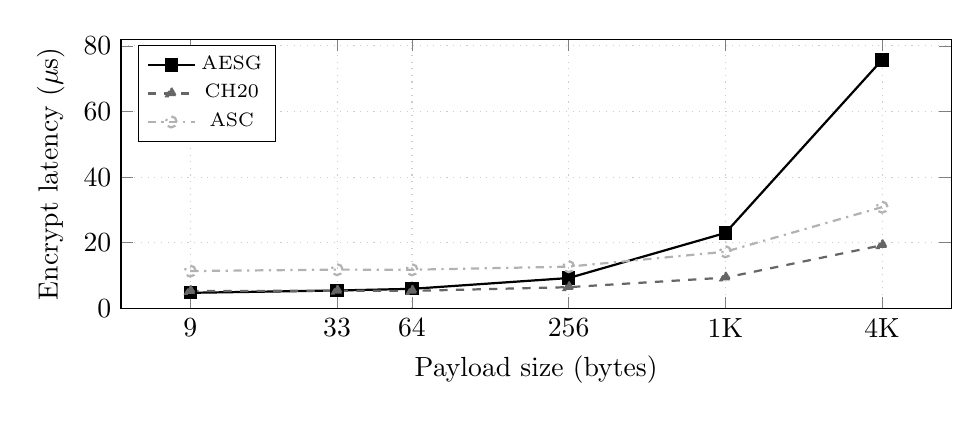
\begin{tikzpicture}
\begin{axis}[
  width=\columnwidth,
  height=5cm,
  xlabel={Payload size (bytes)},
  ylabel={Encrypt latency ($\mu$s)},
  xmode=log,
  log basis x=2,
  xtick={9,33,64,256,1024,4096},
  xticklabels={9,33,64,256,1K,4K},
  ymin=0, ymax=82,
  legend style={at={(0.02,0.98)},anchor=north west,font=\scriptsize},
  grid=major,
  grid style={dotted,gray!40},
  every axis plot/.append style={thick},
  mark size=2pt,
]
\addplot[black, mark=square*]
  coordinates {(9,4.75)(33,5.45)(64,5.96)(256,9.25)(1024,22.98)(4096,75.71)};
\addplot[black!60, mark=triangle*, dashed]
  coordinates {(9,5.30)(33,5.38)(64,5.33)(256,6.47)(1024,9.38)(4096,19.25)};
\addplot[black!30, mark=o, dashdotted]
  coordinates {(9,11.38)(33,11.82)(64,11.78)(256,12.72)(1024,17.27)(4096,30.86)};
\legend{AESG, CH20, ASC}
\end{axis}
\end{tikzpicture}
\caption{AEAD encrypt latency versus payload size.  CH20 (NEON SIMD)
  scales at 3.4\,$\mu$s/KiB; AESG at 17.7\,$\mu$s/KiB (software
  table-lookup).  Below 64\,B, setup cost dominates and ciphers
  converge.}
\label{fig:aead_scaling}
\end{figure}

At 4096\,B the CH20:AESG throughput ratio reaches 3.93$\times$,
while below 64\,B setup cost dominates and the ciphers converge.
The energy-per-bit metric at 256\,B yields
CH20\,=\,21.8\,nJ/bit, AESG\,=\,32.2\,nJ/bit,
ASC\,=\,46.4\,nJ/bit.  For a typical 50\,Hz MAVLink stream
(263\,B packets), per-second AEAD cost ranges from 2.23\,mJ (CH20)
to 4.75\,mJ (ASC)---negligible versus the 3.32\,W board draw.
ChaCha20-Poly1305 is therefore the optimal data-plane cipher for
ARM cores without hardware AES acceleration, delivering 32\% lower
energy per bit than AES-256-GCM.

% =====================================================================
% SECTION 4 — SUITE-LEVEL EVALUATION
% =====================================================================
\subsection{Suite-Level Evaluation}
\label{sec:suite}

Each of the 24 level-matched KEM$\times$SIG combinations was
benchmarked end-to-end on the tunnel prototype (10\,s per suite,
baseline with no DDoS detector).  $T_\text{HS}$ is measured from
handshake initiation to session establishment, including protocol
framing, HKDF key derivation, and Python interpreter overhead.
$T_\text{crypto}$ is the sum of the in-suite KEM and SIG primitive
times recorded during the same run.
Table~\ref{tab:suite} reports all 24 suites grouped by NIST level
(9 at L1, 6 at L3, 9 at L5).

\begin{table*}[t]
\centering
\caption{Measured Suite Handshake Performance --- All 24 Level-Matched KEM$\times$SIG Combinations (Baseline, No DDoS)}
\label{tab:suite}
\footnotesize
\begin{tabular}{@{}llrrrrrl@{}}
\toprule
\textbf{KEM} & \textbf{SIG} &
  \textbf{$T_\text{HS}$} &
  \textbf{$T_\text{crypto}$} &
  \textbf{$\hat{E}_\text{HS}$} &
  \textbf{Crypto} &
  \textbf{$\rho$} & \textbf{Viable?} \\
& & (ms) & (ms) & (mJ) & (\%) & & \\
\midrule
\multicolumn{8}{@{}l}{\textit{NIST Level 1 \normalfont(3~KEMs $\times$ 3~SIGs = 9 suites)}} \\
ML512  & F512   &     12.80 &     5.69 &   44.3 &  44 & 1.0$\times$ & \checkmark \\
ML512  & DSA44  &     14.34 &     2.45 &   49.6 &  17 & 1.1$\times$ & \checkmark \\
HQ128  & F512   &     57.80 &    54.30 &  200   &  94 & 4.5$\times$ & \checkmark \\
HQ128  & DSA44  &     61.43 &    56.50 &  213   &  92 & 4.8$\times$ & \checkmark \\
MC348  & DSA44  &    187.5  &   132.3  &  649   &  71 & 14.6$\times$ & \checkmark$^\star$ \\
MC348  & F512   &    206.1  &   161.4  &  713   &  78 & 16.1$\times$ & \checkmark$^\star$ \\
ML512  & SP128  &    655.1  &   644.8  & 2\,268 &  98 & 51.2$\times$ & $\times$ \\
HQ128  & SP128  &    722.8  &   718.1  & 2\,502 &  99 & 56.5$\times$ & $\times$ \\
MC348  & SP128  &  1\,080   & 1\,045   & 3\,739 &  97 & 84.3$\times$ & $\times$ \\
\midrule
\multicolumn{8}{@{}l}{\textit{NIST Level 3 \normalfont(3~KEMs $\times$ 2~SIGs = 6 suites)}} \\
ML768  & DSA65  &     12.71 &     2.71 &   44.3 &  21 & 1.0$\times$ & \checkmark \\
HQ192  & DSA65  &    155.8  &   159.9  &  543   & 100$^\ddagger$ & 12.3$\times$ & \checkmark$^\star$ \\
MC460  & DSA65  &    257.4  &   185.4  &  897   &  72 & 20.2$\times$ & \checkmark$^\star$ \\
ML768  & SP192  &  1\,250   & 1\,233   & 4\,362 &  99 & 98.3$\times$ & $\times$ \\
HQ192  & SP192  &  1\,537   & 1\,533   & 5\,364 & 100 & 120.9$\times$ & $\times$ \\
MC460  & SP192  & 48\,186$^\dagger$ & ---  & ---   & --- & ---  & $\times$ \\
\midrule
\multicolumn{8}{@{}l}{\textit{NIST Level 5 \normalfont(3~KEMs $\times$ 3~SIGs = 9 suites)}} \\
ML1024 & F1024  &      8.75 &     1.82 &   30.5 &  21 & 1.0$\times$ & \checkmark \\
ML1024 & DSA87  &     16.78 &     2.25 &   58.5 &  13 & 1.9$\times$ & \checkmark \\
HQ256  & F1024  &    271.7  &   283.7  &  947   & 100$^\ddagger$ & 31.1$\times$ & \checkmark$^\star$ \\
HQ256  & DSA87  &    276.1  &   288.9  &  963   & 100$^\ddagger$ & 31.6$\times$ & \checkmark$^\star$ \\
MC8192 & DSA87  &    505.3  &   367.3  & 1\,763 &  73 & 57.7$\times$ & $\times$ \\
MC8192 & F1024  &    678.4  &   527.9  & 2\,367 &  78 & 77.5$\times$ & $\times$ \\
ML1024 & SP256  &  1\,110   & 1\,092   & 3\,873 &  98 & 126.9$\times$ & $\times$ \\
HQ256  & SP256  &  1\,470   & 1\,494   & 5\,128 & 100$^\ddagger$ & 168.0$\times$ & $\times$ \\
MC8192 & SP256  &  1\,651   & 1\,525   & 5\,759 &  92 & 188.7$\times$ & $\times$ \\
\bottomrule
\end{tabular}
\begin{tablenotes}
\footnotesize
\item $T_\text{HS}$: measured end-to-end handshake time (protocol + crypto + overhead).
  $T_\text{crypto}$: sum of in-suite KEM and SIG primitive times.
  $\hat{E}_\text{HS}$: estimated energy ($P_\text{avg} \times T_\text{HS}$, using
    per-primitive $P_\text{avg}$ from Tables~\ref{tab:kem}--\ref{tab:sig}).
  $\rho$: relative to fastest suite at same NIST level.
  Viable: \checkmark\,real-time compatible ($T_\text{HS} < 100$\,ms);
  $\checkmark^\star$\,viable with extended rekey interval;
  $\times$\,non-viable ($T_\text{HS} > 500$\,ms or timeout).
  $^\dagger$Handshake timeout (48.2\,s); crypto fields unavailable.
  $^\ddagger$$T_\text{crypto} > T_\text{HS}$: measurement jitter across
    run boundaries; crypto share capped at 100\%.
\end{tablenotes}
\end{table*}

The default suite (ML768+DSA65) completes a full handshake in
12.71\,ms at Level~3, of which only 2.71\,ms (21\%) is
cryptographic computation; the remaining $\sim$10\,ms is protocol
framing, HKDF key derivation, and interpreter overhead.
At Level~5, ML1024+F1024 measures 8.75\,ms---the fastest of all
24 suites---because Falcon-1024's combined sign+verify (1.18\,ms)
undercuts DSA65 (1.94\,ms) and the crypto share (1.82\,ms) is
minimal.

Three structural observations emerge from the full 24-suite matrix:
(1)~ML-KEM suites are the only family achieving sub-100\,ms
handshakes at every security level ($\rho \leq 1.9\times$);
(2)~SPHINCS$^+$ renders any suite non-viable regardless of KEM
choice, with $T_\text{HS}$ exceeding 655\,ms even paired with
ML-KEM; and (3)~McEliece suites at L5 (MC8192) exceed 500\,ms due
to keygen asymmetry, making them impractical for real-time rekey.
The MC460+SP192 combination timed out at 48.2\,s, confirming that
the MDEAS scheduler's cross-axis constraint forbidding
McEliece$\times$SPHINCS$^+$ pairs is empirically justified.

% =====================================================================
% SECTION 5 — DDoS–CRYPTOGRAPHIC INTERACTION
% =====================================================================
\subsection{DDoS--Cryptographic Interaction}
\label{sec:ddos}

Concurrent DDoS detection competes with the cryptographic pipeline for
CPU and thermal headroom.  All 72 level-matched suites were benchmarked
under baseline (no detector), XGBoost, and TST scenarios
(10\,s per suite per scenario, crypto-only handshakes).\footnote{Both
lightweight detectors use 2~features (\texttt{Mavlink\_Count},
\texttt{Total\_length}), distinct from the 54-feature CIC-IoT-2023
models in Table~\ref{tab:detector_compare}.  TST uses
\texttt{seq\_len=1}; functionally a 3-layer MLP with 1.6\,M
parameters.}

\begin{table}[t]
\centering
\caption{PQC Handshake Overhead Under Concurrent Detection (72~Suites)}
\label{tab:hs_overhead}
\footnotesize
\begin{tabular}{@{}lrr@{}}
\toprule
\textbf{Statistic} & \textbf{XGBoost} & \textbf{TST} \\
\midrule
Mean $\Delta T_\text{HS}$ (\%)   & +2.5   & +71.8  \\
Median $\Delta T_\text{HS}$ (\%) & +0.05  & +32.6  \\
Max $\Delta T_\text{HS}$ (\%)    & +137.2 & +405.1 \\
\midrule
\multicolumn{3}{@{}l}{\textit{Default suite: ML768+AESG+DSA65}} \\
System-level $T_\text{base}$ (ms) & \multicolumn{2}{c}{13.01} \\
$T_\text{HS}$ + detector (ms)   & 13.46  & 37.90  \\
$\Delta T_\text{HS}$ (\%)       & +3.5   & +191.3 \\
\bottomrule
\end{tabular}
\begin{tablenotes}
\footnotesize
\item $\Delta T_\text{HS} = (T_\text{det} - T_\text{base}) / T_\text{base}
  \times 100$.
  $T_\text{base}$ is the measured system-level handshake
  (cf.\ Table~\ref{tab:suite}).
\end{tablenotes}
\end{table}

XGBoost adds a median 0.05\% overhead (mean 2.5\%) to PQC handshakes,
confirming tree-based detection is compatible with real-time
cryptographic operations.  TST nearly triples the default suite
latency (13.01\,$\to$\,37.90\,ms, +191\%), driven by its 93\% CPU
utilization starving the handshake of execution time.

Table~\ref{tab:detector_compare} and Fig.~\ref{fig:detector_cost}
compare the four trained CIC-IoT-2023 detectors on inference cost.

\begin{table}[t]
\centering
\caption{DDoS Detector Inference on RPi4 (CIC-IoT-2023)}
\label{tab:detector_compare}
\footnotesize
\begin{tabular}{@{}lrrrrrr@{}}
\toprule
\textbf{Model} &
  \textbf{Acc.} & \textbf{F1} &
  \textbf{$t_\text{inf}$} & \textbf{P99} &
  \textbf{$\Delta P$} & \textbf{$E_\text{inf}$} \\
& (\%) & & (ms) & (ms) & (mW) & (mJ) \\
\midrule
LightGBM & 93.47$^\dagger$ & 0.937$^\dagger$ & 6.72  & 8.59   & +999  & 29.0  \\
XGBoost  & 94.55$^\dagger$ & 0.947$^\dagger$ & 7.42  & 9.52   & +951  & 31.7  \\
RF       & 93.35$^\dagger$ & 0.935$^\dagger$ & 74.68 & 102.63 & +594  & 291.4 \\
TST      & 90.27$^\dagger$ & 0.80$^\dagger$  & 10.72 & 26.12  & +1\,973 & 56.7 \\
\bottomrule
\end{tabular}
\begin{tablenotes}
\footnotesize
\item $^\dagger$Accuracy and F1 from model documentation; inference
  metrics measured on RPi4 (15\,s per model, idle baseline 3.309\,W).
  CIC-IoT-2023: 3.4\,M samples.
  XGBoost/LightGBM/RF: 54~features, 15~classes.
  TST: 46~features, 6~classes.
\end{tablenotes}
\end{table}

\begin{figure}[t]
\centering
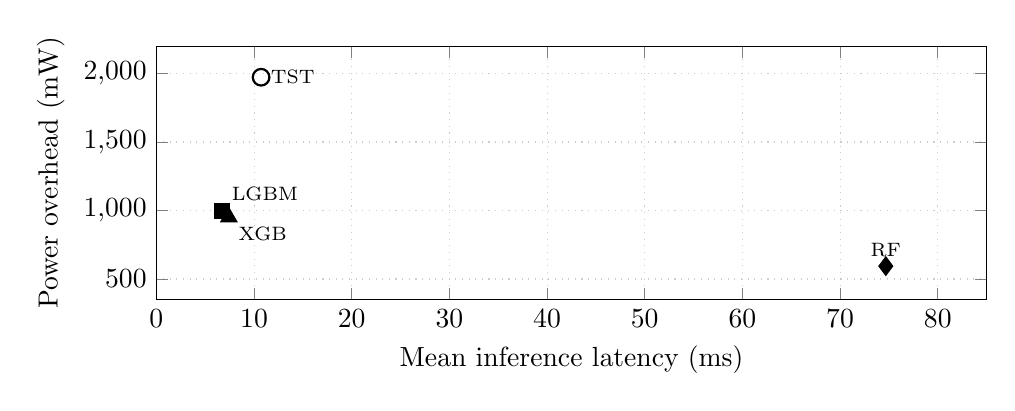
\begin{tikzpicture}
\begin{axis}[
  width=\columnwidth,
  height=4.8cm,
  xlabel={Mean inference latency (ms)},
  ylabel={Power overhead (mW)},
  xmin=0, xmax=85,
  ymin=350, ymax=2200,
  grid=major,
  grid style={dotted,gray!40},
  every axis plot/.append style={thick},
]
\addplot[only marks, mark=square*, mark size=2.5pt, black]
  coordinates {(6.72,999)};
\addplot[only marks, mark=triangle*, mark size=3pt, black]
  coordinates {(7.42,951)};
\addplot[only marks, mark=diamond*, mark size=3pt, black]
  coordinates {(74.68,594)};
\addplot[only marks, mark=o, mark size=3pt, black, thick]
  coordinates {(10.72,1973)};
\node[font=\scriptsize, anchor=south west] at (axis cs:6.72,999) {LGBM};
\node[font=\scriptsize, anchor=north west] at (axis cs:7.42,951) {XGB};
\node[font=\scriptsize, anchor=south] at (axis cs:74.68,594) {RF};
\node[font=\scriptsize, anchor=west] at (axis cs:10.72,1973) {TST};
\end{axis}
\end{tikzpicture}
\caption{Detector resource footprint: inference latency vs.\ power
  overhead.  XGBoost and LightGBM cluster in the low-latency,
  moderate-power region.  RF is a latency outlier (10$\times$);
  TST doubles power draw at modest latency.}
\label{fig:detector_cost}
\end{figure}

XGBoost achieves the highest reported accuracy (94.55\%) at
7.42\,ms mean latency and 31.7\,mJ per inference.
RandomForest consumes $10\times$ more energy (291.4\,mJ) due to its
200-tree ensemble.  TST delivers the lowest accuracy (90.27\%) at
the highest power cost (+1\,973\,mW, 93\% CPU), with a P99 tail of
26.12\,ms indicating variable inference latency.
Tree-based models are therefore the preferred architecture for embedded
PQC--DDoS co-deployment: XGBoost adds negligible handshake overhead
while providing the highest detection accuracy.

% =====================================================================
% SECTION 6 — SCHEDULER BEHAVIORAL IMPACT
% =====================================================================
\subsection{Scheduler Behavioral Impact}
\label{sec:scheduler}

The Multi-Dimensional Energy-Aware Scheduler (MDEAS) manages three
decision axes evaluated at 1\,Hz: (1)~AEAD cipher selection based on
energy and thermal state; (2)~security-level promotion/demotion
triggering PQC rekey; and (3)~DDoS detector activation based on
threat telemetry and thermal headroom.

Each security-level transition requires a complete PQC handshake.
The rekey overhead fraction is:
\begin{equation}
\Phi(R) = \frac{T_\text{HS}}{R + T_\text{HS}}
\label{eq:rekey}
\end{equation}
where $R$ is the rekey interval.  For the default suite ($T_\text{HS} =
12.71$\,ms, Table~\ref{tab:suite}) at the minimum 30\,s interval:
$\Phi = 4.2 \times 10^{-4}$ ($<$0.05\%).  Even the heaviest measured
suite (ML768+SP192, $T_\text{HS} = 1.25$\,s) at 30\,s yields
$\Phi = 0.040$ (4.0\%), confirming that rekey overhead is negligible
for ML-KEM configurations.

Table~\ref{tab:detector_overhead} summarizes the per-detector resource
profiles used for proactive thermal management.

\begin{table}[t]
\centering
\caption{MDEAS Detector Overhead Parameters}
\label{tab:detector_overhead}
\footnotesize
\begin{tabular}{@{}lrrrr@{}}
\toprule
\textbf{Detector} &
  \textbf{$\Delta P$} & \textbf{$\Delta T$} &
  \textbf{$\Delta$CPU} & \textbf{$T_\text{max}$} \\
& (W) & ($^\circ$C) & (pp) & ($^\circ$C) \\
\midrule
None    & 0.00 & 0.0  & 0  & 80.0 \\
XGBoost & 0.95 & 4.8  & 35 & 75.0 \\
TST     & 1.97 & 10.7 & 91 & 69.0 \\
\bottomrule
\end{tabular}
\begin{tablenotes}
\footnotesize
\item $T_\text{max}$: baseline temperature ceiling before detector
  activation is blocked (80$^\circ$C throttle minus $\Delta T$).
  $\Delta$CPU in percentage points.
\end{tablenotes}
\end{table}

The MDEAS enforces cross-axis constraints to prevent pathological
configurations: Ascon-128a is forbidden when TST is active, as its
higher per-packet cost combined with 93\% CPU utilization exceeds the
real-time budget; McEliece KEMs are discouraged under TST due to
CPU-bound keygen contention; all McEliece$\times$SPHINCS$^+$ pairs are
forbidden because $T_\text{HS}$ would exceed the 45\,s rekey timeout;
and detector activation is blocked when temperature exceeds the
per-detector $T_\text{max}$ ceiling.  These constraints reduce the 648
theoretical configurations (216~suites $\times$ 3~detector states) to
approximately 500 viable operating points, navigating the
security--energy--thermal Pareto surface via 1\,Hz telemetry feedback
while guaranteeing the configured minimum security level.
